\documentclass[11pt,oneside]{uhthesis}
%\documentclass[11pt,oneside]{report}
\usepackage{subfigure}
\usepackage[linesnumbered,lined,titlenumbered,ruled]{algorithm2e}
\usepackage{amsmath}
\usepackage{amssymb}
\usepackage{amsbsy}
\usepackage{mathpazo}
\usepackage{float}
\usepackage{braket}
\setlength {\marginparwidth }{3cm}


\usepackage[spanish]{babel}
\usepackage{graphicx}

\usepackage{listings}
\usepackage{color}
\usepackage{booktabs}
\usepackage{multirow}
\usepackage{ragged2e}
\usepackage{multicol}

\floatstyle{ruled}
\restylefloat{table}
\usepackage{listings}
\usepackage{color}

\definecolor{dkgreen}{rgb}{0,0.6,0}
\definecolor{gray}{rgb}{0.2,0,0}
\definecolor{mauve}{rgb}{0.58,0,0.82}

\lstset{language=Lisp,
	aboveskip=10mm,
	belowskip=10mm,
	showstringspaces=false,
	columns=flexible,
	basicstyle={\small\ttfamily},
	keywordstyle=\color{blue},
	commentstyle=\color{dkgreen},
	stringstyle=\color{mauve},
	breaklines=true,
	breakatwhitespace=true,
	tabsize=3,
	numbers=left, numberstyle=\tiny, stepnumber=1,firstnumber=1,
	numbersep=5pt
}

\renewcommand{\tablename}{Tabla}
\title{Enfoques Zero-Shot para la Extracción de Conocimiento a partir de Lenguaje Natural}
\author{Rolando Sánchez Ramos}
\advisor{Dr. Alejandro Piad Morffis}
\degree{Licenciado en Ciencias de la Computación}
\faculty{Facultad de Matemática y Computación}
\date{Noviembre de 2023 \\\vspace{0.25cm}\href{https://github.com/rolysr/nl2ql}{github.com/rolysr/nl2ql}}
\logo{Graphics/uhlogo}

\renewcommand{\vec}[1]{\boldsymbol{#1}}
\newcommand{\diff}[1]{\ensuremath{\mathrm{d}#1}}

\begin{document}
\selectlanguage{spanish}

%\frontmatter
\maketitle

\begin{dedication}
    Dedicación
\end{dedication}
\chapter*{Agradecimientos}\label{chapter:agradecimientos}

Este trabajo constituye la culminación de una trayectoria de estudios que no hubiera sido posible sin el inmenso apoyo de familiares, amigos y colegas de profesión. Quiero en este apartado agradecer a una importante parte de ellas.

	A mis padres, sin los cuales no imagino haber llegado a esta instancia de mi vida. Siempre han estado a mi lado y me han apoyando incondicionalmente en la realización de mis sueños. También, a mis abuelos, cuyo orgullo hacia mí me ha inspirado a mejorar cada día más.

	A mi hermana Angélica y mi hermano Jose Diego, a quienes tengo siempre presentes y con los cuales quiero disfrutar y compartir cada logro que pueda alcanzar.

	A Marian, que con su amor y apoyo ha sido imprescindible para cumplir las metas que me he propuesto y cuya presencia en mi vida me hace sentir afortunado.

	A mis amigos David y Gabriel por estar a mi lado y ser fundamentales para decidirme a estudiar esta carrera. A Andry, por cada trabajo que hicimos juntos y cada vez que criticamos al Barça. A mis amigos Pablo y Abel, por todas las horas que estudiamos juntos y el gusto que daba compartir con ellos tanto dentro como fuera de la universidad. A mi amigo Leandro, por compartir la misma motivación y pasión hacia nuestra profesión. A Marcos, por los momentos compartidos y las dudas que me ayudó a resolver.

	A todos los profesores que tuve en la facultad durante mis años de estudios, en especial al profesor Alejandro Piad, por ser mi modelo a seguir como científico de la computación y como persona. También, al profesor Somoza, por sus conferencias y clases prácticas, las cuales disfruté cada segundo.




\begin{opinion}	
	

\vspace{1cm}


\begin{flushright}
	\underline{\hspace{6.5cm}}\\
	Dr. Alejandro Piad Morffis
	
	Facultad de Matemática y Computación
	
	Universidad de la Habana
	
	Noviembre, 2023
\end{flushright}

\end{opinion}
\begin{resumen}
	Resumen en español
\end{resumen}

\begin{abstract}
	Resumen en inglés
\end{abstract}
\tableofcontents
\listoffigures


%\mainmatter
	
%===================================================================================
% Chapter: Introduction
%===================================================================================
\chapter*{Introducción}\label{chapter:introduction}
\addcontentsline{toc}{chapter}{Introducción}
%===================================================================================

\qquad 

En la época actual, asistimos a un constante aumento en la producción de información en diversos formatos: visual, auditivo y textual, que abarca todos los ámbitos de la sociedad \cite{datagenworld}. De manera particular, resulta sumamente intrigante la información generada a través del ingenio creativo y la investigación humana. Estos tipos de datos se almacenan debido a su relevancia y a la necesidad de acceder a ellos en el futuro, pudiendo optar por una organización estructurada o no. Sorprendentemente, solo alrededor del 20\% de la información a nivel mundial se encuentra estructurada \cite{structdata}.

Las bases de conocimiento constituyen un tipo particular de bases de datos diseñadas para la administración del saber. Estas bases brindan los medios para recolectar, organizar y recuperar digitalmente un conjunto de conocimientos, ideas, conceptos o datos \cite{orgkb}. La ventaja fundamental de mantener la información de manera estructurada radica en su facilidad para ser consultada, ampliada y modificada. Debido a su utilidad y prevalencia, la recuperación de información a través de consultas en bases de conocimiento se ha convertido en una tarea esencial.

Es esencial que la información almacenada en bases de conocimiento adopte un formato adecuado para permitir búsquedas ágiles y precisas. Entre los formatos más comunes se encuentran los modelos de Entidad-Relación y el modelo Relacional. A pesar de ser enfoques más antiguos, el modelo Relacional (BDR) sigue siendo el más ampliamente utilizado en la actualidad \cite{datamodel}. No obstante, en ocasiones, las características específicas del problema demandan un formato más expresivo, y es en este punto donde las bases de datos orientadas a grafos (BDOG) \cite{graphdbs} entran en juego.

Las BDOG han ganado progresivamente popularidad como una manera efectiva de almacenar información en los últimos años. Estas bases tienen la capacidad de modelar una diversidad de situaciones del mundo real al tiempo que mantienen un alto nivel de simplicidad y legibilidad para los seres humanos. Las BDOG presentan numerosas ventajas en comparación con las bases de datos relacionales. Esto incluye un mejor rendimiento, permitiendo el manejo más rápido y eficaz de grandes volúmenes de datos relacionados; flexibilidad, ya que la teoría de grafos en la que se basan las BDOG permite abordar diversos problemas y encontrar soluciones óptimas; y escalabilidad, ya que las bases de datos orientadas a grafos permiten una escalabilidad eficaz al facilitar la incorporación de nuevos nodos y relaciones entre ellos. Ejemplo de un sistema de gestión de BDOG es \textit{Neo4J} \cite{neo4j}, a través del cual es posible construir instancias de este tipo de base de datos e interactuar con las mismas a través del lenguaje de programación \textit{Cypher} \cite{cypher}, el cual posee una sintaxis declarativa similar a \textit{SQL} \cite{sqllang}.

Por otro lado, el avance en la comprensión del lenguaje natural se ha visto potenciado con el surgimiento de los grandes modelos de lenguajes (LLMs) \cite{llms} como GPT-4 \cite{gpt4} o LLaMA-2 \cite{llama2}, los cuales presentan una serie de habilidades emergentes como elaboración de resúmenes de textos, generación de código, razonamiento lógico, traducción lingüística entre otras \cite{llmsskills}. Dichas herramientas constituyen modelos de \textit{Machine Learning} entrenados con un gran volumen de datos, lo cual es posible gracias al número de parámetros con los que estos son configurados \cite{llmsparams}. 

Usualmente, para el uso de los LLMs basta con ofrecerles como dato de entrada un texto (\textit{prompt}), el cual describe la tarea que se espera que estos realicen. Además, son muchas las técnicas existentes para elaborar una entrada de calidad, esto con el objetivo de que la respuesta por parte de dicho modelo de lenguage ofrezca resultados alentadores al respecto, lo cual se conoce como \textit{prompt engineering} \cite{prompengineering}. Una técnica bastánte común es \textit{Zero-Shot Learning} (ZSL) \cite{zeroshotlearning}, la cual consiste en describirle a un LLM un procedimiento a realizar sin ofrecer de antemano ejemplos de cómo resolverlo, como por ejemplo, en tareas relacionadas con la generación de código, donde algunos de estos son capaces de generar algoritmos expresados en un lenguaje de programación formal a partir de una sentencia o consulta en lenguaje natural sin recibir como entrada del usuario algunos ejemplos de código, o especificaciones de cómo funciona el lenguaje objetivo a generar \cite{tex2code1} \cite{text2code2}. 

En lo que respecta a la comprensión del lenguaje natural y su uso en consultas a bases de conocimiento, existen diversas vías llevadas a cabo y con resultados diversos, donde se hacen análisis sintácticos y semánticos sobre la consulta, muchas veces asistidos por diccionarios o mapas sobre la base de conocimiento en cuestión. Se usan modelos de paráfrasis como técnica de aumento de datos y finalmente Transformers \cite{transformers} o incluso LLMs para llevar de la consulta ya curada al lenguaje de consulta formal o a un lenguaje intermedio capaz de expresar a esta a alto nivel \cite{text2sql1} \cite{text2sql2} \cite{text2cypher1} \cite{text2cypher2}.

Por las razones anteriormente expuestas, resulta interesante la investigación sobre la tarea de generación de código de consulta formal a partir de una sentencia en lenguaje natural mediante el uso de LLMs, especialmente el diseño e implementación un experimento capaz de demostrar las capacidades reales de estos para dicho acometido, lo cual designará la importancia de continuar el estudio de dichas herramientas con el objetivo de mejorar los sistemas de extracción de conocimientos en BDOG.

\subsection*{Problemática}
Para utilizar el lenguaje de consulta formal \textit{Cypher} se requiere de conocimientos básicos de programación, lo cual consume cierto tiempo y esfuerzo. Esto tiene como consecuencia que, solo aquellas personas con experiencia en el uso de lenguajes de programación puedan hacer uso de la mayoría de los sistemas de almacenamiento de datos desarrollados con esta tecnología y teniendo en cuenta la necesidad de poseer un conocimiento del dominio sobre el cual está construida la base de datos a consultar. Por lo tanto, llevar a cabo una mejora en las herramientas orientadas a democratizar dicho proceso permitiría hacer más rápido y eficiente dicho proceso de consulta en cuanto a tiempo y recursos computacionales. Debido a dicha situación, se propone una experimentación basada en un LLM capaz de traducir una consulta en lenguaje natural a un código en \textit{Cypher}, donde a su vez se verifique la efectividad de este a partir de enfoques basados en ZSL, los cuales intuitivamente pueden ofrecer como resultado una cota inferior para la efectividad de sistemas desarrollados en base a dichos algoritmos de aprendizaje. Además, actualmente la implementación de sistemas de generación de código de consulta formal está principalmente orientada al lenguaje \textit{SQL}, mientras que para el lenguaje \textit{Cypher}, no existen suficiente estudios recientes que avalen la calidad de tales herramientas para dicho caso de uso. 

\subsection*{Objetivos}
Dadas las ideas anteriores, los objetivos principales del trabajo consistirá en diseñar e implementar una estrategia experimental capaz de evaluar la capacidad mínima de los LLMs para la consulta en lenguaje natural a bases de conocimiento estructuradas con independencia del dominio, para lo cual se empleará un enfoque basado en ZSL.

Para lograr los objetivos generales se trazaron los siguientes objetivos específicos:

\begin{enumerate}
	\item Estudiar el estado del arte de los modelos de Aprendizaje Automático capaces de hacer predicciones de tipo texto-a-texto.
	\item Analizar el trabajo de tesis sobre este tema anteriormente desarrollado en la facultad.
	\item Implementar un modelo de Aprendizaje Automático capaz de convertir una consulta en lenguaje natural humano a un lenguaje formal que permita obtener datos a partir de una 		base de conocimiento.
	\item Explorar las capacidades de enfoques Zero-Shot para la traducción de lenguaje natural al lenguaje Cypher.
	\item Mejorar el sistema de evaluación de resultados permitiendo que el conjunto de datos de prueba y evaluación sea lo más realista posible y con una mayor complejidad.
\end{enumerate}

\subsection*{Organización de la tesis}

[Hablar sobre la estructuracion del documento]




\chapter{Estado del Arte}\label{chapter:state-of-the-art}

\chapter{Propuesta de Solución}\label{chapter: proposedsolution}

En el presente capítulo se abordará la metodología seguida para diseñar el experimento propuesto en este trabajo. Primeramente, se expondrá un marco teórico que formaliza la definición del problema a tratar, esto con el objetivo de presentar los conocimientos base tenidos en cuenta para los enfoques probados. Luego, se detallan los primeros acercamientos desechados \ref{considered_approaches}, argumentando las deficiencias de estos a la hora de arrojar resultados consistentes para la tarea que se desea desarrollar. Finalmente, se detalla la metodología definitiva a implementar, teniendo en cuenta la experiencia obtenida de las anteriores y mostrando su robustez para el análisis experimental.

De forma general, el componente común para cada vía de solución constituye la presencia de un Gran Modelo de Lenguaje, pues representan los modelos más recientes utilizados para la tarea en cuestión; además, ofrecen resultados alentadores para el caso de traducción a lenguaje \textit{SQL} según lo visto en la sección \ref{llm_approach}. Por lo tanto, tiene sentido probar su eficacia para traducir a código en \textit{Cypher}, ya que ambos presentan similitudes como lenguajes formales declarativos para consultar bases de datos. Dicho modelo será analizado como una ``caja negra'' capaz de hacer tareas de traducción de lenguaje natural a una consulta semánticamente equivalente en el lenguaje \textit{Cypher}.

Para cada vía de solución se deberá considerar el despliegue de un sistema de gestión de bases de datos para alguna BDOG, ya que es en este componente donde se almacenará la información a extraer por consultas en un lenguaje orientado a este tipo de almacenamiento. En el caso particular de este trabajo, se considerará el uso de \textit{Neo4J}, con el cual se puede interactuar a partir del lenguaje \textit{Cypher} ya mencionado. Por esto, es importante considerar la implementación de un módulo intermedio para interactuar con una instancia del sistema de gestión \textit{Neo4J}.

El enfoque de \textit{prompt engineering} a utilizar será ZSL, por lo tanto, los textos de entrada que se le darán al modelo para la generación de código \textit{Cypher} no contendrán ejemplos de pares de lenguaje natural con su correspondiente traducción al lenguaje de consulta objetivo. Por lo tanto, se tomarán algunas ideas experimentadas en el estado del arte para \textit{SQL} vistas en el capítulo \ref{chapter: sota}.

\section{Definición del problema \textit{Text-to-Cypher}} \label{problem_definition}
Dentro del ámbito de las bases de datos y las consultas que las acceden, existe una tarea particularmente compleja: traducir preguntas formuladas en lenguaje natural a un lenguaje de consulta estructurado como \textit{Cypher}. Dada una pregunta $Q$, formulada en lenguaje cotidiano, y un esquema de base de datos $S$, el cual se compone a partir del tuplo ${N, A, R}$, donde encontramos múltiples nodos $N$ (que representan instancias de una entidad en la base de datos), atributos $C$ (tanto en nodos como en relaciones) y relaciones entre pares de nodos $R$. La problemática subyacente en el proceso de convertir \textit{Text-to-Cypher} se centra en generar una consulta en lenguaje \textit{Cypher} $Y$ que sea equivalente y responda adecuadamente a la pregunta inicial $Q$ realizada por un usuario humano.

\subsection{LLM para resolver \textit{Text-to-Cypher}} \label{llmfortext2cypher}

Con el auge de la inteligencia artificial y el aprendizaje automático, la tarea de convertir texto en lenguaje natural a código en \textit{Cypher} ha sido recientemente abordada a través de técnicas modernas. En trabajos más recientes, algunos investigadores \cite{sunetal2023} \cite{liuetal2023} han abogado por formular esta tarea como un desafío de generación. Utilizando lo que se conoce como "\textit{prompts}" o indicaciones $P$, es posible dirigir y guiar a un gran modelo de lenguaje $M$ en esta labor. Este modelo, una vez entrenado, puede estimar una distribución de probabilidad sobre posibles consultas \textit{Cypher} $Y$. De esta forma, el modelo es capaz de generar, paso a paso y token por token, una consulta apropiada.

La fórmula subyacente para generar la consulta $Y$ se estructura como:
$$P_M(Y|P, S, Q) = \prod_{i=1}^{|Y|}{P_M(Y_i | P, S, Q, Y < i)}$$ \label{llm_query_generation}

Para simplificar, $Y< i$ se refiere al fragmento inicial o prefijo de la consulta \textit{Cypher} que se está construyendo. Mientras que $P_M(Yi|*)$ denota la probabilidad condicional asociada con la generación del i-ésimo token, considerando factores como el prefijo existente $Y<i$, la indicación $P$, el esquema $S$ y la pregunta original $Q$.

Uno de los hallazgos más reveladores en el campo reciente es el concepto de aprendizaje en contexto (ICL, por sus siglas en inglés) \cite{llmsoverview}, en el cual, grandes modelos de lenguaje pueden adaptarse y aprender de unos pocos ejemplos presentados en un contexto específico. Esta estrategia, defendida por varios investigadores \cite{sunetal2023} \cite{pourrezandrafiei2023}, ha mostrado que los LLMs pueden abordar y dominar una amplia variedad de tareas complejas con una cantidad limitada de datos. Sin embargo, hay un equilibrio que mantener: agregar más ejemplos conlleva un aumento en los costos, tanto en términos de mano de obra para preparar esos ejemplos como en términos de costos de procesamiento y tokens al interactuar con APIs avanzadas como la de OpenAI \cite{openaiapikey}. En este estudio, el foco recae en trabajar eficientemente con indicaciones al modelo de lenguaje sin requerir ejemplos adicionales.

\section{Enfoques considerados} \label{considered_approaches}

El desarrollo de un sistema con un LLM (\textit{Large Language Model}) para hacer inferencias de \textit{Zero-Shot} y generar \textit{Cypher} implica varios enfoques y desafíos. A continuación, se detallan los enfoques considerados y las dificultades encontradas.

Primero, se exploraron modelos de código abierto. El primer modelo probado fue \texttt{Alpaca Lora 7B} \cite{alpacalora}. Sin embargo, la calidad de las inferencias no fue la adecuada. En algunos casos, las respuestas eran \textit{Cypher} no compilable con errores de sintaxis. En otros casos, el modelo generaba otro lenguaje de consulta que no era \textit{Cypher}, como por ejemplo \textit{SQL}. Posteriormente, se probó con \texttt{GPT4All} \cite{gpt4all} y con \texttt{Vicuna 7B} \cite{vicuna7b}, obteniendo resultados similares. Estos modelos, aunque útiles, no proporcionaban la precisión y la generación de \textit{Cypher} que se requería para el sistema.

Además, se consideró la posibilidad de entrenar un propio modelo de lenguaje grande con muchos parámetros para tareas específicas. Este modelo podría ser capaz de generar \textit{Cypher} sin haber sido entrenado específicamente para eso. Sin embargo, esta opción fue descartada debido a la inviabilidad total. Entrenar un modelo de lenguaje grande requiere una gran cantidad de recursos de computación \cite{llmsoverview}. Además, la tarea de entrenar un modelo para generar \textit{Cypher} sin haber sido entrenado específicamente para eso es extremadamente desafiante. Aunque técnicamente posible, requeriría una inversión significativa de tiempo y recursos, así como un conocimiento profundo de los modelos de lenguaje y el aprendizaje profundo.

En resumen, el desarrollo de un sistema con un LLM para hacer inferencias de \textit{Zero-Shot} y generar \textit{Cypher} implica una serie de desafíos. Estos incluyen la elección del modelo correcto, la necesidad de entrenar el modelo para generar \textit{Cypher} específicamente, y la inversión significativa de recursos y tiempo. A pesar de estos desafíos, el uso de LLMs ofrece la promesa de generar \textit{Cypher} de manera eficiente y precisa, lo que puede ser de gran utilidad en una variedad de aplicaciones.

\section{Propuesta de solución diseñada} \label{designed_proposal}

En el desarrollo de sistemas de bases de datos, la interacción eficiente y la gestión de esquemas son fundamentales para la manipulación y el mantenimiento de datos. En este contexto, se ha desarrollado una arquitectura de software compuesta por varios componentes interconectados diseñados para interactuar con una base de datos de grafos, con especial atención en \textit{Neo4J}, un sistema de manejo de bases de datos basado en grafos.

Uno de los componentes clave de esta arquitectura es el \texttt{GraphContractor}, un módulo diseñado para facilitar la interacción con la base de datos. Este componente actúa como intermediario entre la aplicación y la base de datos, manejando la lógica necesaria para establecer conexiones, ejecutar consultas y manejar los resultados. La modularidad del \texttt{GraphContractor} permite su reutilización y fácil mantenimiento, además de proporcionar una capa de abstracción que simplifica las operaciones de la base de datos para los desarrolladores.

Para la generación de esquemas de la base de datos, se ha creado el \texttt{SchemaMaker}, una herramienta automatizada que se encarga de construir los esquemas necesarios para \textit{Neo4J}. Esta herramienta juega un rol crucial en la estructuración de la base de datos, ya que define la organización de nodos, relaciones, propiedades y restricciones. El \texttt{SchemaMaker} garantiza que la base de datos esté correctamente configurada para cumplir con los requisitos del dominio y las necesidades de la aplicación, asegurando así la integridad y coherencia de los datos.

En la interfaz entre el lenguaje natural y la base de datos, se ha integrado el modelo de lenguaje \texttt{GPT-4}, utilizado como una ''caja negra'' para la traducción de consultas en lenguaje natural a \textit{Cypher}, el lenguaje de consulta para \textit{Neo4J}. La capacidad de \texttt{GPT-4} para comprender y generar texto hace posible que los usuarios realicen consultas complejas sin necesidad de conocer la sintaxis específica de \textit{Cypher}. Para mejorar la precisión y relevancia de las traducciones, se ha elaborado una plantilla de prompt que se nutre de la salida del \texttt{SchemaMaker}. Esta plantilla guía al modelo de lenguaje proporcionando contexto y estructura, lo que permite que \texttt{GPT-4} genere consultas \textit{Cypher} más precisas y eficientes.

Finalmente, se ha desarrollado el \texttt{DBSeeder}, un componente encargado de poblar la base de datos de \textit{Neo4J} con datos iniciales o de prueba. Utilizando consultas \textit{Cypher} generadas por el modelo de lenguaje \texttt{GPT-4}, el \texttt{DBSeeder} trabaja en conjunto con el \texttt{GraphContractor} para insertar nodos, atributos y relaciones en la base de datos. Esta funcionalidad es especialmente valiosa en las etapas de desarrollo y prueba, donde se requiere de una base de datos poblada para validar el diseño y la lógica de la aplicación. Además, el \texttt{DBSeeder} está diseñado para operar dentro de un contenedor de \textit{Docker}, lo que ofrece ventajas significativas en términos de portabilidad, escalabilidad y aislamiento del entorno de desarrollo.

Cada uno de estos componentes representa un eslabón en la cadena de herramientas que permitirán interactuar con la base de datos de grafos de manera más intuitiva y automatizada. La integración de tecnologías avanzadas como \texttt{GPT-4} en el proceso no solo mejora la accesibilidad para los usuarios finales sino que también agiliza el ciclo de desarrollo, ofreciendo un enfoque moderno y eficiente en la gestión de bases de datos de grafos como \textit{Neo4J}.

\subsection{Interacción con una base de datos \textit{Neo4J}} \label{graph_contractor}

El componente \texttt{GraphContractor} actúa como un facilitador o intermediario entre el usuario y la base de datos \textit{Neo4J}. Su propósito es simplificar las tareas de conexión y ejecución de consultas contra la base de datos, manejando internamente los detalles de la comunicación y posibles excepciones.

Al instanciar \texttt{GraphContractor}, se le proporciona una URL, junto con un nombre de usuario y contraseña para la autenticación. Luego, esta herramienta intenta establecer una conexión con la instancia de la base de datos \textit{Neo4J} en la URL especificada. Si la conexión es exitosa, el \texttt{GraphContractor} estará listo para ejecutar consultas. Si la conexión falla, por ejemplo, debido a problemas con la red o las credenciales de acceso, se informará al usuario al respecto con un mensaje informativo.

Una vez que el \texttt{GraphContractor} está conectado a la base de datos, es posible realizar consultas a una base de datos objetivo. Para dicha tarea, este acepta una cadena de texto que representa la consulta \textit{Cypher} a ejecutar. Al efectuar dicha funcionalidad con una consulta de \textit{Cypher} válida, \texttt{GraphContractor} la ejecutará en la base de datos y devolverá los resultados. Si ocurre algún error durante la ejecución de la consulta, como una sintaxis incorrecta de \textit{Cypher} o un problema de conexión, el error se capturará y se presentará al usuario, ofreciendo retroalimentación inmediata.

\begin{figure}[H]\label{gcimage}
	\centering
	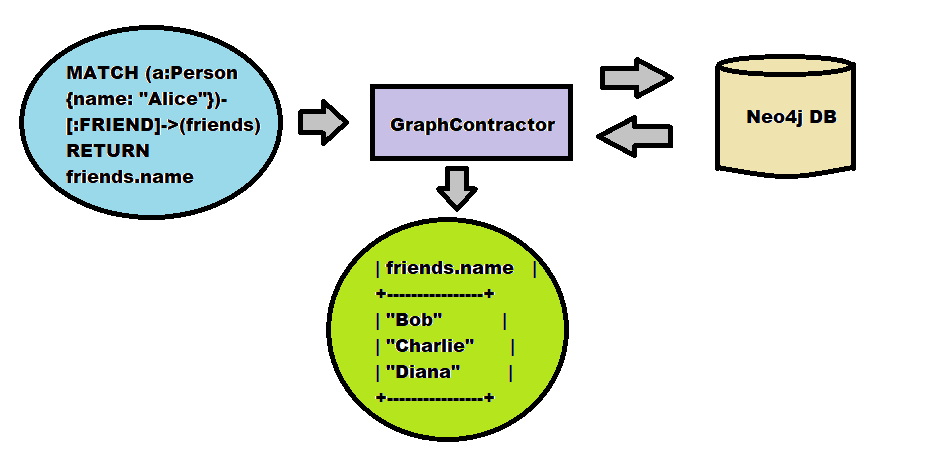
\includegraphics[width = 0.9\textwidth]{./Graphics/graph_contractor}
	\caption{Flujo de funcionamiento del componente \texttt{GraphContractor}.}
\end{figure}

En resumen, \texttt{GraphContractor} encapsula la complejidad de la gestión de la conexión a la base de datos y la ejecución de consultas, proporcionando una interfaz simplificada para interactuar con \textit{Neo4J}. Esto permite a los usuarios centrarse en la lógica de sus consultas y manejo de datos, en lugar de en los detalles subyacentes de la implementación de la base de datos.

\subsection{Extracción de información de una base de datos \textit{Neo4J}} \label{knowledge_base}

En el ámbito de la extracción de información de bases de datos orientadas a grafos, como \textit{Neo4J}, se ha desarrollado un componente denominado \texttt{KnowledgeBase}. Este componente actúa como una interfaz avanzada para la interacción con dichas bases de datos, aprovechando las capacidades del componente \texttt{GraphContractor}. La funcionalidad principal de \texttt{KnowledgeBase} radica en su habilidad para encapsular consultas predefinidas en el lenguaje \textit{Cypher}, el cual es específico para bases de datos \textit{Neo4J}.

El diseño de \texttt{KnowledgeBase} tiene como objetivo principal facilitar la extracción de información de manera eficiente y transparente. Para lograr esto, utiliza consultas en \textit{Cypher} que están integradas dentro de sus funcionalidades. Estas consultas son ejecutadas a través de una instancia interna de \texttt{GraphContractor}, proporcionando una capa de abstracción que simplifica las interacciones del usuario con la base de datos.

Sus funcionalidades principales implementadas fueron:

\begin{itemize}
\item \textbf{Inicialización y Configuración}: El proceso de inicialización establece una conexión vital con la base de datos y prepara el componente para operaciones de consulta. Esto implica la integración con un sistema central que maneja las interacciones con la base de datos.

\item \textbf{Verificación de Existencia de Entidades}: Una funcionalidad central permite verificar la presencia de entidades específicas en la base de datos. Se emplean etiquetas y propiedades para formular consultas que determinan la existencia de la entidad.

\item \textbf{Comprobación de Atributos en Entidades}: Otra capacidad importante es determinar si una entidad posee un atributo específico. Esta función es clave para validar la integridad y completitud de los datos.

\item \textbf{Extracción y Análisis de Entidades y Atributos}: La extracción de etiquetas de entidades provee una visión general de los tipos de datos almacenados. Adicionalmente, se realiza un análisis detallado de los atributos asociados con cada entidad y relación, incluyendo el tipo de dato y los rangos de valores.

\item \textbf{Inferencia del Tipo de Dato}: La habilidad para identificar el tipo de dato de un valor proporcionado es esencial para el manejo adecuado de los datos, permitiendo realizar conversiones y validaciones de tipo cuando sea necesario.

\item \textbf{Identificación de Claves y Atributos}: Se realizan operaciones para extraer claves de entidades y relaciones. Esto proporciona información detallada sobre los campos disponibles en diferentes tipos de nodos y enlaces.

\item \textbf{Análisis de Relaciones entre Entidades}: Identificar y catalogar las relaciones entre distintas entidades es crucial para comprender las interacciones y conexiones dentro de la base de datos.
\end{itemize}

\begin{figure}[H]\label{dbseeder}
	\centering
	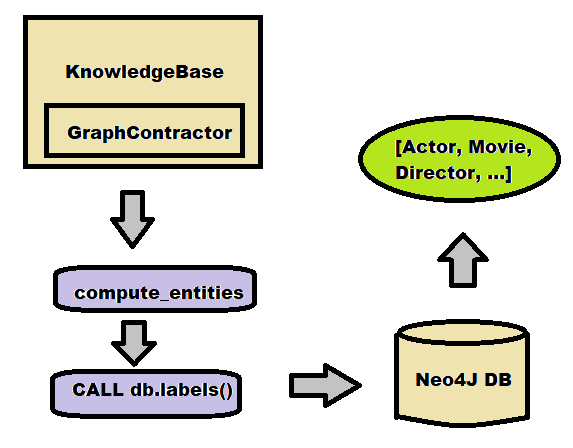
\includegraphics[width = 0.9\textwidth]{./Graphics/knowledgebase}
	\caption{Flujo de funcionamiento del componente \texttt{KnowledgeBase}.}
\end{figure}

\subsection{Almacenamiento de información en una base de datos \textit{Neo4J}} \label{dbseeding}

El componente \texttt{DBSeeder} es una herramienta diseñada para cargar datos en una base de datos en forma de grafo. Su propósito es automatizar el proceso de toma de datos estructurados y su inserción en la base de datos, creando nodos y relaciones entre ellos según se define en los datos de entrada. La interacción de este con una instancia de una base de datos \textit{Neo4J} es a través de una instancia del componente \texttt{KnowledgeBase} visto en la sección \ref{knowledge_base}.

Al inicializar esta herramienta, se le proporcionan dos piezas de información esenciales: un conjunto de conocimientos que describe la estructura de la base de datos y una ruta a un archivo que contiene los datos a ser sembrados en la base de datos. Estos datos de entrada son esenciales para guiar el proceso de sembrado.

Una vez configurada, la herramienta tiene la capacidad de procesar los datos de entrada. Esto se realiza leyendo cada línea del archivo de datos, donde cada línea representa un conjunto de información que debe ser transformada en elementos dentro de la base de datos. La herramienta analiza cada línea para comprender y aislar las partes que corresponden a entidades y las relaciones entre ellas.

Para cada conjunto de datos, la herramienta verifica si los elementos ya existen en la base de datos. Si no es así, procede a crear nuevos nodos que representan entidades y luego establece relaciones entre estos nodos, basándose en la relación especificada en los datos.

\begin{figure}[H]\label{dbseeder}
	\centering
	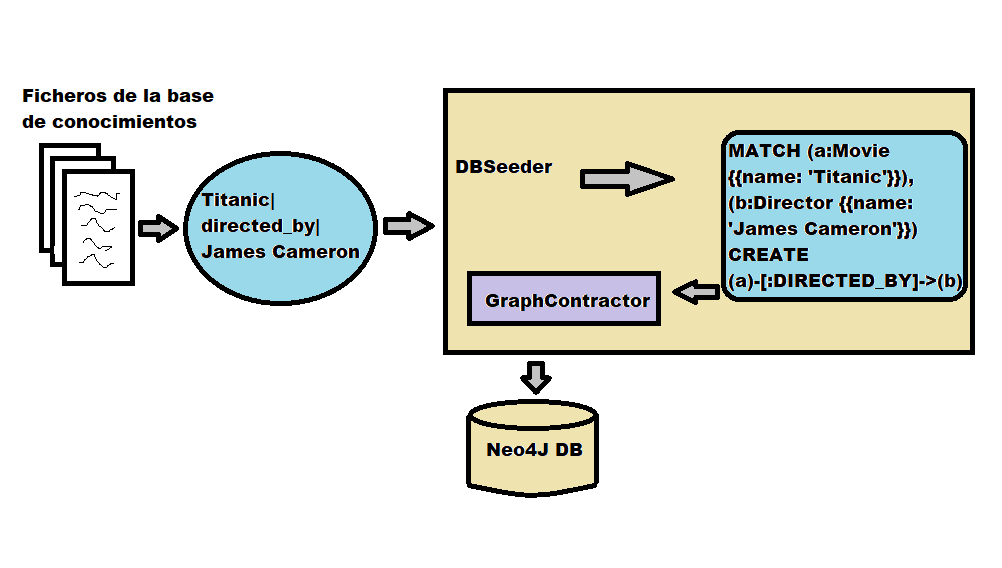
\includegraphics[width = 0.9\textwidth]{./Graphics/dbseeder}
	\caption{Flujo de funcionamiento del componente \texttt{DBSeeder}.}
\end{figure}

El proceso de llenado en la base de datos asegura que no se introduzcan duplicados y que los datos se estructuren correctamente esta la base de datos de acuerdo con sus reglas y definiciones. Al finalizar, la base de datos debería reflejar una red de nodos interconectados que representan tanto las entidades como las relaciones definidas en el archivo de datos original. Este proceso es fundamental para preparar la base de datos para su uso en aplicaciones que requieren acceso a datos relacionales y estructurados en forma de grafo.

\subsection{Selección del modelo} \label{model_selection}

La selección de \texttt{GPT-4} para la generación de código a partir de lenguaje natural utilizando aprendizaje \textit{Zero-Shot} (ZSL) está justificada por varias razones fundamentadas en investigaciones y comparaciones técnicas recientes.  \texttt{GPT-4} es un avance significativo respecto a sus predecesores, construido sobre la arquitectura de \texttt{GPT-3} pero alcanzando nuevos niveles de rendimiento y escala \cite{gpt4}. Este modelo mejora en la corrección factual de las respuestas y reduce las alucinaciones, donde el modelo comete errores de hecho o razonamiento, obteniendo un $40\%$ más de precisión que  \texttt{GPT-3.5} en las pruebas de rendimiento factual internas de OpenAI \cite{gpt4}.

El modelo  \texttt{GPT-4} se basa en la arquitectura Transformer, que utiliza mecanismos de atención para procesar texto, y se ha mejorado con una mezcla de expertos (MoE) para lograr un modelo con aproximadamente $1.76$ billones de parámetros, un orden de magnitud mayor que  \texttt{GPT-3} \cite{gpt4}. Además, estudios recientes han mostrado que \texttt{GPT-4} supera a  \texttt{GPT-3.5} en aprendizaje zero-shot en casi todas las tareas evaluadas, lo que incluye una variedad de dominios de razonamiento como deductivo, inductivo, abductivo, analógico, causal y multi-salto, a través de tareas de preguntas y respuestas \cite{gpt4}.

Además, el modelo  \texttt{GPT-4} emplea técnicas de \textit{fine-tuning} y Aprendizaje por Refuerzo con Retroalimentación Humana (RLHF), lo que le permite ser un modelo multimodal robusto capaz de procesar entradas textuales y visuales y generar salidas basadas en texto \cite{gpt4}. Este enfoque ha demostrado ser eficaz en la mejora de las capacidades de razonamiento de los modelos de lenguaje grandes (LLMs), lo que lo hace especialmente adecuado para tareas complejas que requieren razonamiento, como la traducción de lenguaje natural a lenguaje de consulta formal \cite{gpt4all}.

\begin{table}[H]
  \centering
  \caption{Rendimiento de GPT-4 en referencias académicas. \cite{gpt4}}
  \begin{tabularx}{\textwidth}{Xcccc}
    \toprule
    & \textbf{GPT-4} & \textbf{GPT-3.5} & \textbf{LM SOTA} & \textbf{SOTA} \\
    \midrule
    \textbf{MMLU} & 86.4\% & 70.0\% & 70.7\% & 75.2\% \\
    \textbf{HellaSwag} & 95.3\% & 85.5\% & 84.2\% & 85.6\% \\
    \textbf{AI2 Reasoning Challenge (ARC)} & 96.3\% & 85.2\% & 85.2\% & 86.5\% \\
    \textbf{WinoGrande} & 87.5\% & 81.6\% & 85.1\% & 85.1\% \\
    \textbf{HumanEval} & 67.0\% & 48.1\% & 26.2\% & 65.8\% \\
    \textbf{DROP} & 80.9\% & 64.1\% & 70.8\% & 88.4\% \\
    \textbf{GSM-8K} & 92.0\% & 57.1\% & 58.8\% & 87.3\% \\
    \bottomrule
  \end{tabularx}
  \label{tab:my_label}
\end{table}

En comparación con otros modelos como \texttt{PALM, Chinchilla, LaMDA, LLaMA} y \texttt{Gopher}, que también han evaluado sus habilidades de razonamiento,  \texttt{GPT-4} se destaca por su capacidad mejorada de aprendizaje zero-shot y por el uso de estrategias de prompting refinadas para mejorar aún más su rendimiento en tareas de razonamiento, lo que lo convierte en una elección prometedora para la generación de código \cite{gpt4}.

\begin{figure}[H]\label{simplegpt4}
	\centering
	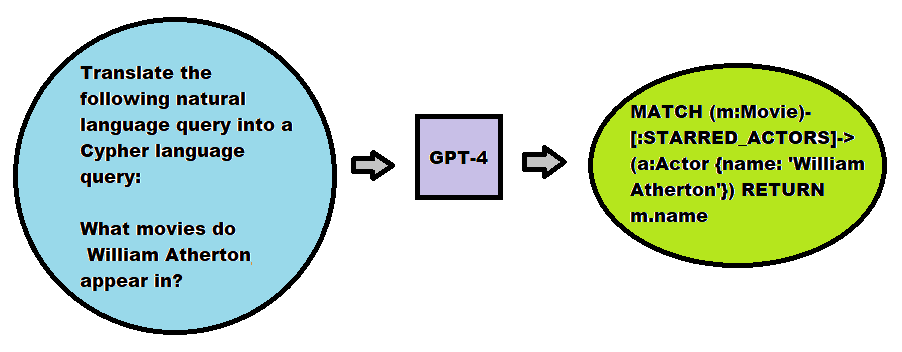
\includegraphics[width = 0.9\textwidth]{./Graphics/simplegpt4use}
	\caption{Ejemplo básico sobré como utilizar \texttt{GPT-4} para traducir lenguaje natural en lenguaje de consulta \textit{Cypher}.}
\end{figure}

\subsection{Diseño de la información entrada al LLM} \label{prompt_design}

Tal y como se mostró en la sección anterior, el uso de \texttt{GPT-4} para la tarea de traducción no resulta complicado, pues este es utilizado como una gran ``caja negra'' capaz de realizar operaciones que se le indiquen en un texto (\textit{prompt}) de entrada. Debido a esto, también es importante mencionar que no cualquier entrada es efectiva o suficiente para obtener el resultado esperado por lo cual, al proceso de diseñar una entrada de calidad para que el modelo realice una tarea específica exitosamente se denomida \textit{prompt engineering} \cite{promptengineering}. 

Dado que la hipótesis central de este trabajo se basa en el uso del aprendizaje \textit{Zero-Shot} (ZSL), el texto de entrada al modelo \texttt{GPT-4} no puede contener ejemplos de cómo traducir una consulta en lenguaje humano a lenguaje \textit{Cypher}, es decir, no deberá reflejar contenido demostrativo de la tarea a realizar, lo cual se justifica por la misma definición del enfoque ZSL \cite{zeroshotlearning}. Además, como parte de la información de entrada al modelo para este tipo de tareas, es común añadir una descripción de la estructura de la base de datos a consultar \cite{text2sql1}, lo cual se conoce como esquema de la base de datos \cite{dbschema}. 

Por lo mencionado anteriormente, el texto de entrada al modelo deberá contener:

\begin{itemize}
	\item \textbf{La tarea a ejecutar}: Se le describirá al modelo la tarea a realizar, mencionando los datos que recibirá de entrada y el formato en que se desea obtener la respuesta.
	\item \textbf{Esquema de la base de datos}: Se especificará el contenido de la base de datos objetivo en forma de grafo, mencionando las entidades, relaciones (especificando si son en una sola o ambas direcciones entre un par de entidades) y atributos presentes en la misma (correspondientes tanto a las entidades como a las relaciones entre estas).
	\item \textbf{Consulta en lenguaje natural}: En este caso, se añadirá la consulta en lenguaje natural humano a traducir.
\end{itemize}

Para la obtención del esquema de la base de datos de tipo \textit{Neo4J} se diseñó el componente \texttt{SchemaMaker}. Con el fin de elaborar la descripción de la estructura de la fuente de datos objetivo, este recibe los nombres de las entidades, las relaciones y los atributos presentes en la misma. Dicha información la obtiene auxiliándose del componente \texttt{KnowlegdeBase} analizado en la sección \ref{knowledge_base}, mediante el cual se realizan las consultas en lenguaje \textit{Cypher} pertinentes a la instancia de la fuente de datos \textit{Neo4J} en cuestión. A continuación se muestra un ejemplo del funcionamiento de la herramienta \texttt{SchemaMaker}:

\begin{figure}[H]\label{schemamaker}
	\centering
	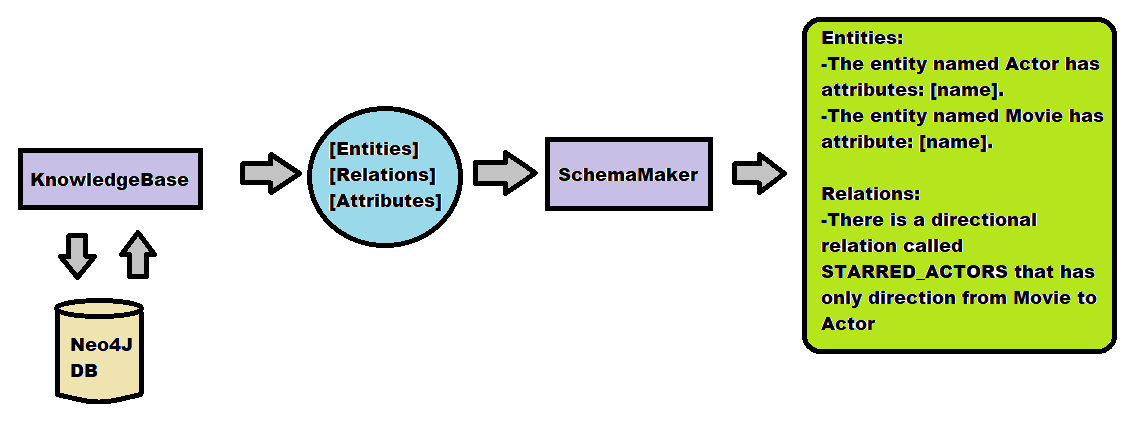
\includegraphics[width = 0.9\textwidth]{./Graphics/schemamaker}
	\caption{Ejemplo del proceso que se realiza para obtener un formato verbalizado de una base de datos \textit{Neo4J} con el uso del \texttt{SchemaMaker}.}
\end{figure}

Finalmente, el texto de entrada para el modelo a utilizar mencionado en la sección \ref{model_selection} se integraría de la siguiente manera al proceso de traducción de lenguaje natural a lenguaje \textit{Cypher}:

\begin{figure}[H]\label{completeinoutgpt4}
	\centering
	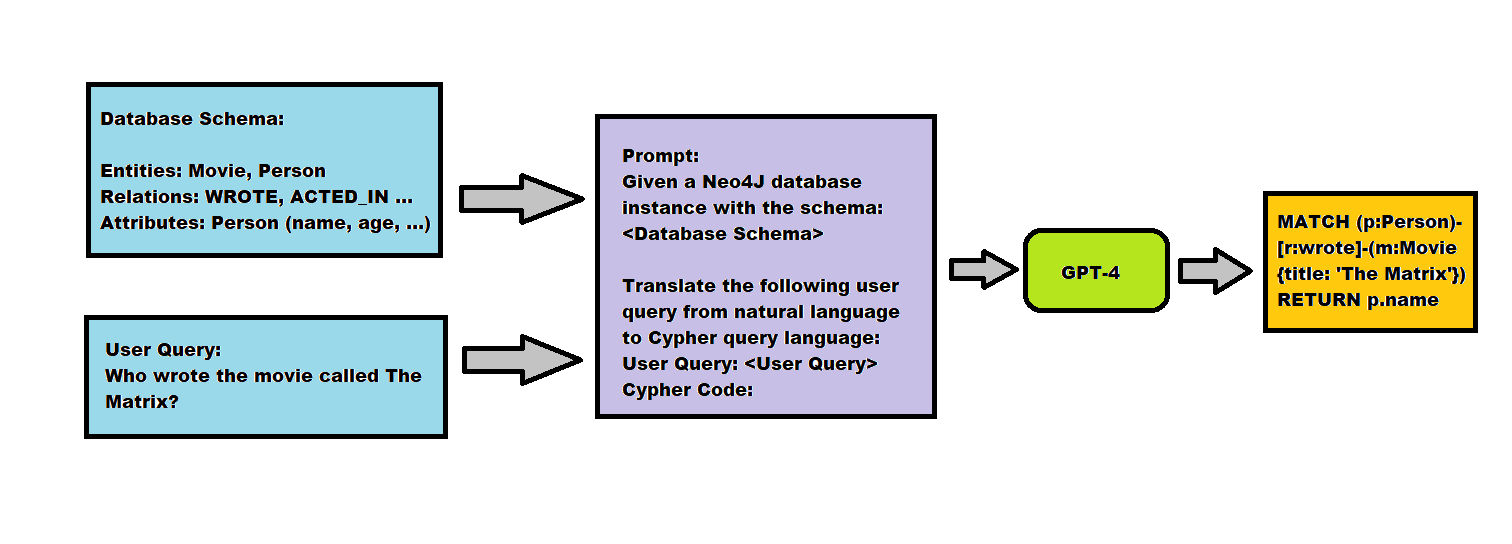
\includegraphics[width = 1\textwidth]{./Graphics/inoutgpt4}
	\caption{Flujo de entrada y salida en el proceso de traducción de lenguaje natural a código en \textit{Cypher}.}
\end{figure}

Tal y como se muestra en la imagen anterior, junto con la entrada de una consulta en lenguaje natural se elabora un texto de entrada al modelo utilizando además, el esquema de la base de datos \textit{Neo4J} a consultar, la cual como ya se mencionó en esta subsección, es producida por el \texttt{SchemaMaker}.

\subsection{Caso de estudio} \label{sample_case}

A partir de los contenidos abordados en esta sección, resulta importante mostrar la arquitectura general del sistema diseñado, así como el flujo de funcionamiento de la misma.

\begin{figure}[H]
	\centering
	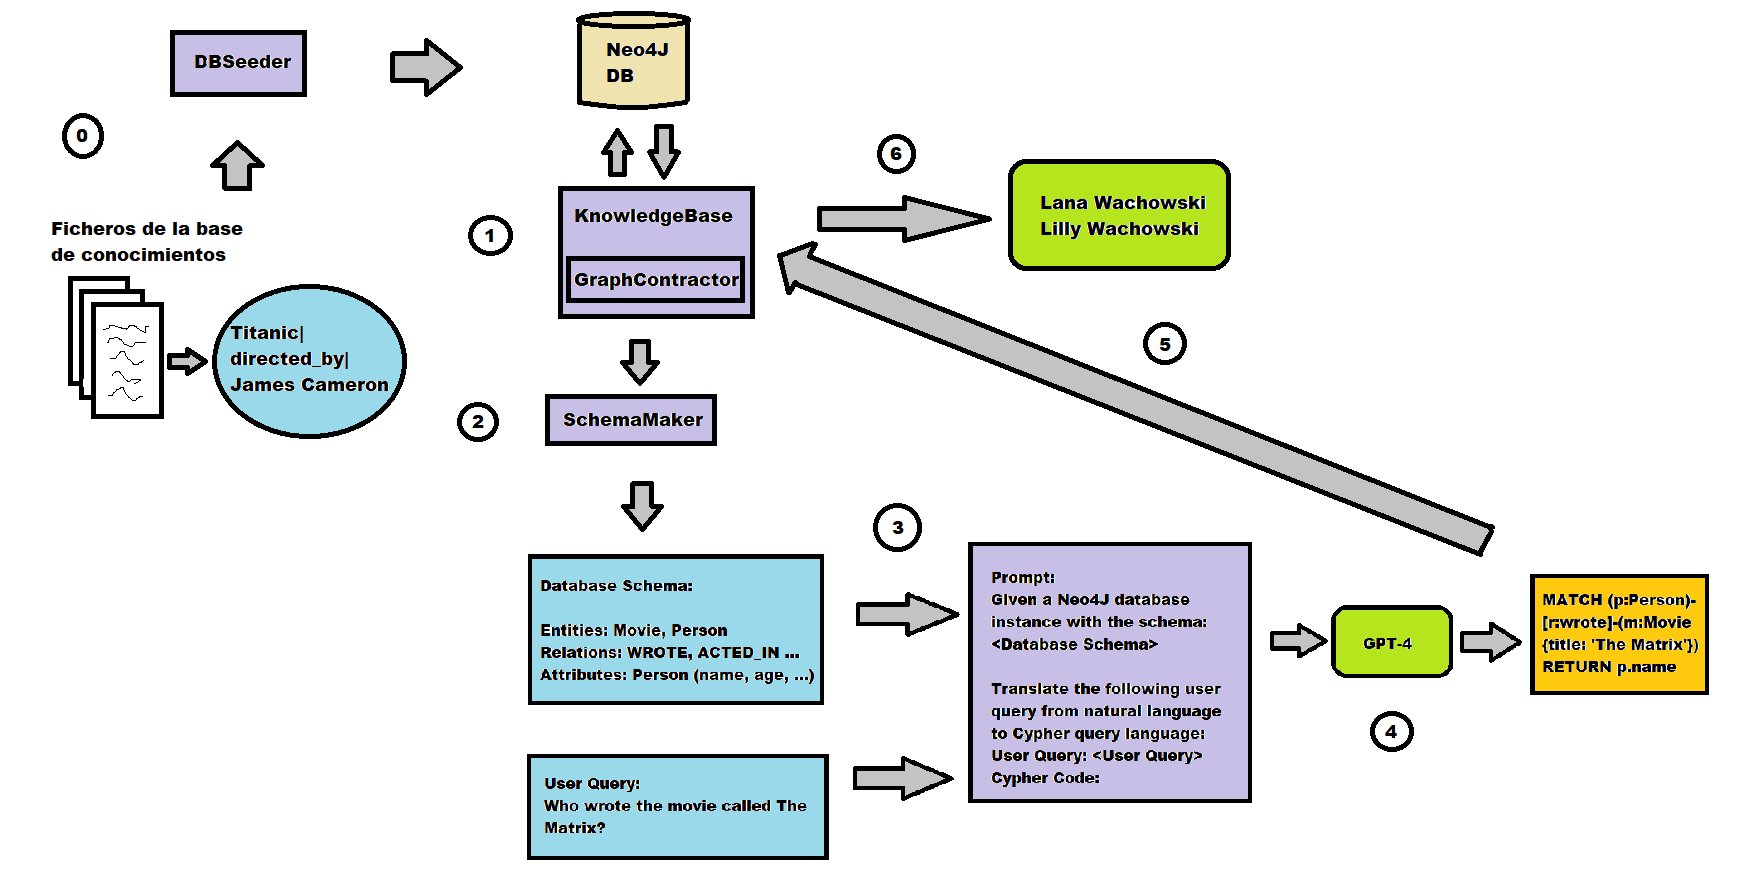
\includegraphics[width = 1.05\textwidth]{./Graphics/case_of_study}
	\caption{Arquitectura y funcionamiento de la propuesta de solución.}
\end{figure}\label{fig:caseofstudy}

Para una mejor comprensión de la figura \ref{fig:caseofstudy} se añadieron un conjunto de íncides que resaltan las distintas fases por las que pasa el sistema implementado. A continuación se enumeran y explican en qué consisten cada una de estas etapas:

\begin{enumerate} \label{pipeline_algorithm}

\item \textbf{Paso 0}: Este representa el proceso mediante el cual se construye una instancia de una base de datos \textit{Neo4J}  a partir de un conjunto de ficheros de texto. Esta tarea se puede llevar a cabo mediante el componente \texttt{DBSeeder}, el cual puede programarse con funcionalidades específicas de acuerdo al formato de los ficheros iniciales y los datos que estos contienen. Como se mencionó en la sección \ref{dbseeder}, el componente \texttt{DBSeeder} se apoya del componete \texttt{GraphContractor} internamente para realizar peticiones a la base de datos con el objetivo de añadir nuevos registros de información, traduciendo la creación de entidades, relaciones y atributos en instrucciones de \textit{Cypher} ejecutadas sobre una base de datos \textit{Neo4J} objetivo.

\item \textbf{Paso 1}: En esta fase, el componente \texttt{KnowledgeBase} extrae la información referente a las entidades, relaciones y atributos de una base de datos \textit{Neo4J} existente. Para ello, hace uso internamente de una instancia de un \texttt{GraphContractor} \ref{graph_contractor}.

\item \textbf{Paso 2}: En este paso, se utiliza la herramienta \texttt{SchemaMaker} \ref{schemamaker}, el cual recibe la información de la base de datos procedente del componente \texttt{KnowledgeBase} y produce una descripción verbalizada y legible en lenguaje natural sobre la estructura de la instancia de \textit{Neo4J} objetivo.

\item \textbf{Paso 3}: En este momento del proceso general, se recibe una consulta descrita en lenguaje natural humano sobre una solicitud de datos de la base de datos objetivo. Luego esta es utilizada junto con el esquema de la base de datos obtenido del \texttt{SchemaMaker}  para conformar un texto de entrada al modelo \texttt{GPT-4} con las características mencionadas en la sección \ref{prompt_design}.

\item \textbf{Paso 4}: Una vez obtenido el texto de entrada para realizar una inferencia con el modelo \texttt{GPT-4}, se procede a hacer una ejecución de este, produciendo así como salida un texto que representa un código en lenguaje \textit{Cypher}.

\item \textbf{Paso 5}: En esta etapa, se utiliza la salida del modelo \texttt{GPT-4} para ser ejecutada sobre la base de datos \textit{Neo4J} objetivo mediante la herramienta \texttt{KnowledgeBase}.

\item \textbf{Paso 6}: Finalmente, se obtiene la respuesta procedente de la base de datos \textit{Neo4J} con la información solicitada.

Con lo anteriormente explicado se expone un ejemplo de caso de uso donde se tienen como entradas al sistema una instancia de una base de datos \textit{Neo4J} y una consulta en lenguaje humano para obtener como salida final el conjunto de datos extraídos de dicha base de datos objetivo correspondientes a la solicitud textual dada sobre estos.

\end{enumerate}

\chapter{Detalles de Implementación}\label{chapter: implementation}

En este capítulo se exponen los detalles sobre la implementación de los componentes que intervinieron en el proyecto, resaltando los principales aspectos de programación tenidos en cuenta.

El sistema implementado fue desarrollado con el \textit{IDE} \textit{VSCode} \cite{vscode}, el cual fue configurado para utilizar el lenguaje \textit{Python} (versión 3.9) \cite{python} y contar con las facilidades que esta herramienta ofrece para detectar errores de sintaxis y de dependencias en tiempo de compilación. Por otro lado, el sistema operativo utilizado para implementar el proyecto fue \textit{Ubuntu-22.04}, con el cual se facilitó el proceso de instalación de bibliotecas para el lenguaje de programación empleado.

En general, no se optó por utilizar una arquitectura de software específica, ya que el objetivo del proyecto se centra fundamentalmente en utilizar el sistema resultante para evaluar los experimentos orientados a responder la hipótesis de estudio y no en desarrollar una aplicación a ser llevada a producción para emplearse por usuarios humanos.

\section{Despliegue de una instancia de una base de datos \textit{Neo4J}}

Para iniciar una instancia de una base de datos en forma de grafo de tipo \textit{Neo4J} se utilizó \textit{Docker} \cite{docker}, con el cual se desplegó un contenedor que pudiese ejecutar el sistema de gestión de \textit{Neo4J} y ser accesible ante peticiones de una aplicación mediante el protocolo \textit{Bolt} \cite{boltprotocol}.

Una vez intalado \textit{Docker} se utilizó el siguiente comando:

\begin{figure}[H]
\begin{lstlisting}[language=bash]
 docker run \
--name testneo4j \
-p 7474:7474 -p 7687:7687 \
-d \
-v $HOME/neo4j/data:/data \
-v $HOME/neo4j/logs:/logs \
-e NEO4J_AUTH=neo4j/testpassword \
neo4j
\end{lstlisting}
\caption{Comando utilizado para desplegar una base de datos \textit{Neo4J}.}
\end{figure}

Este comando ejecuta un contenedor de \textit{Docker} con la imagen de \textit{Neo4J}, expone los puertos 7474 y 7687, guarda los datos y los registros en el \textit{host}, y establece las credenciales de autenticación para la interfaz de usuario de \textit{Neo4J}:

\begin{itemize}

    \item \textbf{--name testneo4j}: Esta opción asigna el nombre \textit{testneo4j} al contenedor a ejecutar.

   	\item \textbf{-p 7474:7474 -p 7687:7687}: Estas opciones hacen corresponder los puertos 7474 y 7687 del contenedor a los mismos puertos del \textit{host}. Esto permite acceder a los servicios que se ejecutan en estos puertos dentro del contenedor desde el \textit{host}.

    \item \textbf{-d}: Esta opción hace que el contenedor se ejecute en segundo plano (modo \textit{detached}).

    \item \textbf{-v $HOME/neo4j/data:/data -v $HOME/neo4j/logs:/logs}: Estas opciones montan los directorios $HOME/neo4j/data y $HOME/neo4j/logs del \textit{host} en los directorios \textit{/data} y \textit{/logs} del contenedor, respectivamente. Esto permite que los datos y los registros generados por el contenedor se guarden en el \textit{host}.

    \item \textbf{-e NEO4J\_AUTH=neo4j/testpassword}: Esta opción establece la variable de entorno \texttt{NEO4J\_AUTH} en el contenedor con el valor \textit{neo4j/testpassword}. Esto se utiliza para configurar la autenticación en \textit{Neo4J}.

    \item \textbf{neo4j}: Esta es la imagen de la que se está creando el contenedor. En este caso, se está utilizando la imagen oficial de \textit{Neo4J}.

\end{itemize}

\section{\texttt{GraphContractor}}

Para la implementación del componente \texttt{GraphContractor} se diseñó una clase para interactuar con una instancia de base de datos \textit{Neo4J}. La clase hereda de la clase \texttt{Graph} del módulo \texttt{py2neo}, que proporciona una interfaz de alto nivel para interactuar con bases de datos \textit{Neo4J}.

\begin{figure}[H]
\begin{lstlisting}[language=python]
class GraphContractor(Graph):
    """
        Graph Contractor class for interacting with a Neo4J DB instance
    """

    def __init__(self, url, name, password):
        try:
            self.graph = Graph(url, auth=(name, password))

        except Exception as e:
            print(e)
            print('Error connecting to the database(Remember VPN)')

    def make_query(self, query: str):
        try:
            return self.graph.run(query).data()
        except BaseException as e:
            print(e)
            return str(e)
\end{lstlisting}
\caption{Implementación de la clase \texttt{GraphContractor}.}
\end{figure}

La clase GraphContractor tiene un método \texttt{\_\_init\_\_} que se utiliza para inicializar una nueva instancia de la clase. Este método toma tres argumentos: \texttt{url, name} y \texttt{password}, que se utilizan para establecer una conexión con la base de datos \textit{Neo4J}. Esta clase también tiene un método \texttt{make\_query} que se utiliza para ejecutar consultas en la base de datos \textit{Neo4J}. Este método toma una consulta como una cadena de texto y la ejecuta en la base de datos.

\section{\texttt{KnowledgeBase}}

El componente \texttt{KnowledgeBase} fue implementado en una clase cuyo constructor recibe una instancia de una entidad de tipo \texttt{GraphContractor}:

\begin{figure}[H]
\begin{lstlisting}[language=python]
class KnowledgeBase:
	def __init__(self, graph: GraphContractor) -> None:
        self.graph = graph

    def entity_exists(self, label, property_name, property_value):
    	...
	def entity_has_attribute(self, label, property_name, entity_name):
    	...

	def compute_entities(self):
        ent = self.graph.graph.run('CALL db.labels()')
        entities = QueryUtils._unfold_graph_resp(ent)
        return entities

	def compute_attributes(self, entities, relations):
		...
	def compute_relations(self, entities):
		...
	def _infer_data_type(self, value):
		...
	def get_type_min_max_entity_attribute(self, entity, attribute_name):
		...
	def get_type_min_max_relation_attribute(self, relation, attribute_name):
		...
	def get_keys_of_label(self, label):
		...
	def get_keys_of_relation(self, relation):
		...
\end{lstlisting}
\caption{Implementación de la clase \texttt{KnowledgeBase}.}
\label{code:kbimage}
\end{figure}

Esta herramienta presenta un conjunto de métodos auxiliares para diversas tareas que impliquen la extracción de información de una base de datos, donde cada uno internamente utiliza la instancia del \texttt{GraphContractor} proporcionado. Por ejemplo, tal como se muestra en la figura \ref{code:kbimage}, para obtener el conjunto de entidades de la base de datos se ejecuta un código de \textit{Cypher} correspondiente sobre la instancia de \textit{Neo4J} a consultar.

\section{\texttt{DBSeeder}}

La clase \texttt{DBSeeder} en el código proporcionado en la figura \ref{code:dbseeder} se utiliza para poblar (\textit{seed}) una base de datos con información en algún formato específico y una base de conocimientos de tipo \textit{Neo4J}.

\begin{figure}[H]
\begin{lstlisting}[language=python]
class DBSeeder:
	def __init__(self, kb: KnowledgeBase, db_base_file_path: str) -> None:
        self.kb = kb
        self.db_base_file_path = db_base_file_path

    def seed_db(self):
		...
	def create_entities_relations_attributes(self, entity1, relation_type, entity2):
		...
\end{lstlisting}
\caption{Implementación de la clase \texttt{DBSeeder}.}
\label{code:dbseeder}
\end{figure}

El método constructor \texttt{\_\_init\_\_} recibe dos argumentos: \texttt{kb}, que es una instancia de \texttt{KnowledgeBase}, y \texttt{db\_base\_file\_path}, que es la ruta del archivo de la base de datos base. Por otro lado, el método \texttt{seed\_db} se encarga de almacenar información en la base de datos objetivo. Este método abre el el conjunto de ficheros que contienen información de la base de datos para su lectura y luego itera sobre cada línea del archivo, llamando al método \texttt{create\_entities\_relations\_attributes}, el cual verifica si las entidades \texttt{entity1} y \texttt{entity2} existen en la base de datos. Si no existen, se crean. Luego, se crea una relación entre el par de entidades dadas y la relación especificada.


\section{\texttt{SchemaMaker}}

En la figura \ref{code:schemamaker} se muestra la implementación de la clase \texttt{SchemaMaker}, la cual tiene el método estático \texttt{compute\_schema\_description}. 

\begin{figure}[H]
\begin{lstlisting}[language=python]
class SchemaMaker:    
    @staticmethod
    def compute_schema_description(entities, relations, attributes):
        schema_description = ""
        schema_description += f"Entities: {entities}\n"
        for entity in entities:
            entity_attrs = attributes[entity]
            if len(entity_attrs) > 0:
                schema_description += f"The entity named {entity} has the attributes: {[attr[0] for attr in entity_attrs]}\n"
        for relation in relations:
            for ent1, ent2, is_double_sense in relations[relation]: 
                if is_double_sense:
                    schema_description += f"There is a relation called {relation} between the entitites {ent1} and {ent2}. The relation {relation} can be used in both senses.\n"
                    continue
                schema_description += f"There is a directional relation called {relation} that has only direction from {ent1} to {ent2}.\n"
            if len(attributes[relation]) > 0:
                schema_description += f"The relation {relation} has attributes {attributes[relation]}\n"
        return schema_description
\end{lstlisting}
\caption{Implementación de la clase \texttt{Schema Maker}.}
\label{code:schemamaker}
\end{figure}

Dicho método toma tres argumentos: \texttt{entities}, \texttt{relations} y \texttt{attributes}, los cuales utiliza para generar una descripción del esquema de una base de datos. Este comienza inicializando una cadena vacía \texttt{schema\_description} y luego agrega información sobre las entidades y relaciones. Primero, agrega una línea que indica las entidades presentes en el esquema. Luego, para cada entidad, si tiene atributos, agrega una línea que indica los atributos de esa entidad. Después de manejar las entidades, el método pasa a las relaciones. Para cada relación, si es de doble sentido, agrega una línea que indica que existe una relación bidireccional entre las dos entidades involucradas. Si no es de doble sentido, agrega una línea que indica que existe una relación unidireccional desde la primera entidad a la segunda. Finalmente, si la relación tiene atributos, agrega una línea que indica los atributos de la relación.

\section{\texttt{GPT-4}}

Para implementar una estructura capaz de realizar inferencias a partir del modelo \texttt{GPT-4} se utilizó la biblioteca \textit{Langchain} y se definió una función \texttt{get\_model} que se utiliza para inicializar un modelo de lenguaje basado en el tipo especificado. Fue necesario además, el uso de una \texttt{API\_KEY} de \textit{OpenAI} con el objetivo de acceder a los modelos disponibles \cite{openaiapikey}.

La función \texttt{get\_model} toma dos argumentos: \texttt{model\_type} y \texttt{model\_name}. La variable \texttt{model\_type} puede ser chat o cualquier otro tipo de modelo, y \texttt{model\_name} es el nombre del modelo específico que se va a utilizar. Para el caso específico de este trabajo el tipo de modelo fue chat y el nombre utilizado fue gpt-4, mientras que la temperatura del modelo utilizada fue $0.7$.

Primero, la función inicializa una plantilla de \textit{prompt} de acuerdo a si el modelo a utilizar es de tipo chat o generativo. La plantilla de \textit{prompt} se inicializa con un texto predefinido que describe la tarea del modelo y los marcadores de posición para el lenguaje de consulta, el tipo de base de datos, el esquema y la consulta. Luego, la función inicializa un modelo de lenguaje basado en \texttt{model\_type}. Ambos modelos se inicializan con un nombre de modelo y una temperatura. Finalmente, la función inicializa una instancia de un modelo capaz de hacer inferencias a partir de un texto de entrada predefinido con variables.

\begin{figure}[H]
\begin{lstlisting}[language=python]
from langchain.prompts import PromptTemplate, ChatPromptTemplate
from langchain.chat_models import ChatOpenAI
from langchain import LLMChain
from langchain import OpenAI

# template for the model
template = """
You are an agent capable of transforming natural language queries to queries in the query language {query_language}. Your task is: Given a database schema of type {database_type} and a query written in human natural language, return only the code to answer that query in the query language {query_language} and respect the relations directions.

The database schema is: {schema}

The natural language query is: {query}

The code in the query language {query_language} is:

""".strip()

def get_model(model_type, model_name):
    # Init prompt template
    prompt = ChatPromptTemplate.from_template(template=template) if model_type == "chat" else PromptTemplate(template=template, input_variables=[
        "query_language", "database_type", "schema", "query"])
    
    # Init llm
    llm = ChatOpenAI(model=model_name, temperature=0.7) if model_type == "chat" else OpenAI(temperature=0.7)

    # Init chain
    llm_chain = LLMChain(prompt=prompt, llm=llm)

    return llm_chain
\end{lstlisting}
\caption{Implementación para utilizar el modelo \texttt{GPT-4}.}
\label{code:schemamaker}
\end{figure}
\chapter{Análisis Experimental}\label{chapter: experiment}

En este capítulo se presentan los marcos experimentales utilizados para evaluar la efectividad del sistema propuesto en el capítulo \ref{chapter: proposedsolution} para la traducción de una consulta en lenguaje natural al lenguaje de consulta formal \textit{Cypher}. Cada enfoque utilizado consistió en el uso de un conjunto de tuplas que contenían en común una consulta en lenguaje natural de ejemplo a traducir hacia un segundo elemento correspondiente con un objetivo a medir en la traducción.

Todos los experimentos fueron ejecutados en un servidor privado virtual (\textit{VPS}) \label{used_machine} con sistema operativo \textit{Ubuntu-20.04}, memoria \textit{RAM} de 16Gb, una \textit{CPU} AMD basada en la arquitectura \textit{x86\_64}, con 8 núcleos y una velocidad de 2649.998 MHz y con un ancho de banda de 16Mb/s para la comunicación con servicios como la \textit{API} de \textit{OpenAI}.

El sistema de evaluación fue desarrollado sobre el \textit{benchmark MetaQA} \ref{classic_metaqa}, el cual constituye el principal conjunto de datos de evaluación para la tarea \textit{Text-to-Cypher} vista en la sección \ref{problem_definition}. En este caso se utilizó la versión clásica, donde los pares de evaluación consistían en una consulta en lenguaje natural con su correspondiente respuesta en la base de datos.

\section{Evaluación sobre el \textit{benchmark} \textit{MetaQA} \cite{metaqa}} \label{classic_metaqa}
\textit{MetaQA} \cite{metaqa} es un conjunto de datos diseñado para la tarea de razonamiento de múltiples pasos (\textit{multi-hop}) en respuesta a preguntas. Está compuesto por entidades, relaciones y preguntas en lenguaje natural relacionadas con películas. Cada nodo en el grafo de conocimientos representa una entidad (como una película, actor o director), y las aristas representan relaciones entre las entidades. El conjunto de datos también incluye preguntas a tres niveles de complejidad (\textit{1-hop,} \textit{2-hop} y \textit{3-hop}), con cada nivel requiriendo razonamiento sobre un número creciente de aristas en la base de datos en forma de grafos analizada. A continuación se muestra un ejemplo de la distribución de dicho conjunto de datos:

\begin{table}[h]
\centering
\begin{tabular}{|c|r|r|r|}
\hline
 & \textbf{1-hop} & \textbf{2-hop} & \textbf{3-hop} \\ \hline
\textbf{Train} & 96,106 & 118,980 & 114,196 \\ \hline
\textbf{Dev} & 9,992 & 14,872 & 14,274 \\ \hline
\textbf{Test} & 9,947 & 14,872 & 14,274 \\ \hline
\end{tabular}
\caption{Distribución de los conjuntos de datos del \textit{benchmark MetaQA}.}
\label{tab:metaqatable}
\end{table}

En este estudio solo se utilizarán los datos referentes a los conjuntos de evaluación (\texttt{Test}) para cada uno de los grupos especificados, ya que el modelo empleado es un gran modelo de lenguaje mediante la técnica \textit{Zero-Shot}, por lo que no es necesario hacer un proceso de entrenamiento al mismo para realizar la tarea en cuestión.

Las principales métricas de evaluación utilizadas fueron el número de consultas que al ser traducidas a \textit{Cypher} y ser ejecutadas ejecutadas sobre la base de conocimiento daban una respuesta idéntica a la respuesta objetivo (\texttt{correct}), así como el porcierto de dichas consultas acertadas (\texttt{correct\%}) sobre el total de consulta (\texttt{n}), número de consultas compiladas con éxito y su porciento correspondiente (\texttt{compiled} y \texttt{compiled\%} respectivamente), algunas relacionadas con los recursos consumidos para el experimento como el costo monetatrio (\texttt{cost} (USD)) y el tiempo de ejecución de la evaluación en segundos (\texttt{elapsed\_seconds}). También, se calculó eficacia del modelo con respecto a cada tipo de consulta en el conjunto de evaluación y medidas clásicas como la precisión, el recobrado y la medida $F1$ para evaluar la calidad de la extracción de información. La métrica \texttt{correct\%} fue la utilizada para comparar el resultado del modelo empleado sobre otros resultados en el estado del arte \cite{gpt4all}. Además, implícitamente, al evaluar la efectividad del modelo sobre las consultas de los conjuntos de evaluación de \textit{1-hop, 2-hop} y \textit{3-hop}, se evalúa la eficacia del modelo sobre consultas que requieren de una relación, dos relaciones y hasta tres relaciones de conexión respectivamente para encontrar la respuesta a la consulta.

Para la preparación del conjunto de datos se insertaron los elementos correspondientes a la base de conocimientos en una instancia de \textit{Neo4J} con ayuda del componente \texttt{DBSeeder} visto en la sección \ref{dbseeder}. Luego se tomaron los conjuntos de prueba (\textit{Test}) para \textit{1-hop, 2-hop} y \textit{3-hop} y para cada par de evaluación se ejecutó el procedimiento descrito en el listado \ref{pipeline_algorithm}.

\subsection{Resultados}

Los resultados obtenidos para cada métrica analizada para cada conjunto de evaluación se muestran en la siguiente figura:

\begin{table}[H]
\centering
\begin{tabular}{|c|c|c|c|c|c|}
\hline
 & \textbf{n} & \textbf{compiled} & \textbf{correct} & \textbf{compiled\%} & \textbf{correct\%} \\ \hline
\textbf{hop 1} & 9947 & 9386  & 7613 & 94.36 & 76.53  \\ \hline
\textbf{hop 2} & 14872 & 13733  & 6462 & 92.34  & 43.45  \\ \hline
\textbf{hop 3} & 14274 & 13221  & 4430 & 92.62 & 31.03  \\ \hline
\end{tabular}
\caption{Resultados de ejecutar \texttt{GPT-4} en los conjuntos de datos de prueba de \textit{MetaQA} para \textit{hop1, hop2} y \textit{hop3}.}
\label{tab:results1}
\end{table}

En la tabla \ref{tab:results1} se muestran los resultados de eficacia del modelo \texttt{GPT-4} para traducir consultas a \textit{Cypher} tal que puedan ser utilizadas para extraer información de la base de datos objetivo. En este caso, una consulta generada por el sistema utilizado fue considerada eficaz si al ejecutar el código de \textit{Cypher} sobre la base de datos correspondiente, dicho resultado coincide con los datos de respuesta esperados asociados a cada par de los conjuntos de evaluación. Para aquellas consultas cuyo código de \textit{Cypher} correspondiente requería de la presencia de una relacion específica entre dos entidades en cuestión se tuvo relevante resultado del $76.53\%$ de acierto. Por otro lado, aquellas consultas que requerían de la generación de una consulta con dos y haste tres relaciones tuvieron como resultados unos discretos $43.45\%$ y $31.03\%$ respectivamente, lo que nos indica la deficiencia de este modelo para responder expresiones en lenguaje natural complejas que requieran acceder a la información de más una relación entre dos entes de la base de datos en forma de grafo.

Es importante resaltar de los resultados anteriores la efectividad del sistema para generar consultas de \textit{Cypher} compilables, donde para cada lote de evaluación se obtuvieron valores sobre el $92\%$, lo que confirmar que se tuvo éxito en la inmensa mayoría de las veces que el modelo trató de traducir la consulta inicial en lenguaje natural a solamente un texto conteniendo un código de \textit{Cypher}. En los casos donde dicho suceso no fue posible, se debió principalmente a que el modelo generó un texto adicional describiendo la consulta, ofrecía más de una consulta o simplemente había un error sintáctico en el código.

\begin{table}[H]
\centering
\begin{tabular}{|c|c|c|c|}
\hline
\textbf{Tipo de consulta} & \textbf{Correctas} & \textbf{Total} & \textbf{Efectividad} \\ \hline
\textbf{actor\_to\_movie} & 650 & 879 & 73.94 \\ \hline
\textbf{director\_to\_movie} & 446 & 553 & 80.65 \\ \hline
\textbf{movie\_to\_actor} & 672 & 1105 & 60.81 \\ \hline
\textbf{movie\_to\_director} & 984 & 1301 & 75.63 \\ \hline
\textbf{movie\_to\_genre} & 946 & 1143 & 82.76 \\ \hline
\textbf{movie\_to\_language} & 251 & 294 & 85.37 \\ \hline
\textbf{movie\_to\_tags} & 611 & 846 & 72.22 \\ \hline
\textbf{movie\_to\_writer} & 909 & 1091 & 83.31 \\ \hline
\textbf{movie\_to\_year} & 1122 & 1420 & 79.01 \\ \hline
\textbf{tag\_to\_movie} & 236 & 411 & 57.42 \\ \hline
\textbf{writer\_to\_movie} & 786 & 904 & 86.94 \\ \hline
\end{tabular}
\caption{Resultados para las consultas del lote \textit{hop 1}.}
\label{tab:results3}
\end{table}

\begin{longtable}{|c|c|c|c|}
\caption{Resultados para las consultas del lote \textit{hop 2}.} \\
\hline
\textbf{Tipo de consulta} & \textbf{Correctas} & \textbf{Total} & {\textbf{Efectividad}} \\ \hline
\endfirsthead
\multicolumn{4}{c}%
{{\bfseries \tablename\ \thetable{} --  continuación desde la página anterior }} \\
\hline
\textbf{Tipo de consulta} & \textbf{Correctas} & \textbf{Total} & {\textbf{Efectividad}} \\ \hline
\endhead
\hline \multicolumn{4}{|r|}{{Continuación en la siguiente página}} \\ \hline
\endfoot
\hline \hline
\endlastfoot
\textbf{actor\_to\_movie\_to\_director} & 488 & 929 & 52.53 \\ \hline
\textbf{director\_to\_movie\_to\_director} & 86 & 164 & 52.44 \\ \hline
\textbf{director\_to\_movie\_to\_language} & 160 & 193 & 82.90 \\ \hline
\textbf{writer\_to\_movie\_to\_writer} & 481 & 763 & 63.04 \\ \hline
\textbf{actor\_to\_movie\_to\_genre} & 470 & 823 & 57.11 \\ \hline
\textbf{director\_to\_movie\_to\_genre} & 380 & 533 & 71.30 \\ \hline
\textbf{actor\_to\_movie\_to\_actor} & 585 & 971 & 60.25 \\ \hline
\textbf{writer\_to\_movie\_to\_actor} & 414 & 838 & 49.40 \\ \hline
\textbf{actor\_to\_movie\_to\_writer} & 417 & 834 & 50.00 \\ \hline
\textbf{movie\_to\_director\_to\_movie} & 501 & 1081 & 46.35 \\ \hline
\textbf{actor\_to\_movie\_to\_year} & 186 & 985 & 18.88 \\ \hline
\textbf{writer\_to\_movie\_to\_genre} & 550 & 844 & 65.17 \\ \hline
\textbf{director\_to\_movie\_to\_actor} & 300 & 483 & 62.11 \\ \hline
\textbf{movie\_to\_actor\_to\_movie} & 254 & 1180 & 21.53 \\ \hline
\textbf{writer\_to\_movie\_to\_year} & 45 & 1020 & 4.41 \\ \hline
\textbf{director\_to\_movie\_to\_year} & 138 & 594 & 23.23 \\ \hline
\textbf{director\_to\_movie\_to\_writer} & 107 & 402 & 26.62 \\ \hline
\textbf{movie\_to\_writer\_to\_movie} & 225 & 896 & 25.11 \\ \hline
\textbf{writer\_to\_movie\_to\_director} & 380 & 763 & 49.80 \\ \hline
\textbf{writer\_to\_movie\_to\_language} & 133 & 250 & 53.20 \\ \hline
\textbf{actor\_to\_movie\_to\_language} & 162 & 326 & 49.70 \\ \hline
\end{longtable}
\label{tab:results4} 

\begin{longtable}{|c|c|c|c|}
\caption{Resultados para las consultas del lote \textit{hop 3}.} \\
\hline
\textbf{Tipo de consulta} & \textbf{Correctas} & \textbf{Total} & {\textbf{Efectividad}} \\ \hline
\endfirsthead
\multicolumn{4}{c}%
{{\bfseries \tablename\ \thetable{} --  continuación desde la página anterior }} \\
\hline
\textbf{Tipo de consulta} & \textbf{Correctas} & \textbf{Total} & {\textbf{Efectividad}} \\ \hline
\endhead
\hline \multicolumn{4}{|r|}{{Continuación en la siguiente página}} \\ \hline
\endfoot
\hline \hline
\endlastfoot
\textbf{movie\_to\_director\_to\_movie\_to\_language} & 132 & 616 & 21.43 \\ \hline
\textbf{movie\_to\_director\_to\_movie\_to\_actor} & 147 & 1069 & 13.75 \\ \hline
\textbf{movie\_to\_actor\_to\_movie\_to\_language} & 377 & 840 & 44.88 \\ \hline
\textbf{movie\_to\_writer\_to\_movie\_to\_year} & 256 & 833 & 30.73 \\ \hline
\textbf{movie\_to\_actor\_to\_movie\_to\_director} & 609 & 1166 & 52.23 \\ \hline
\textbf{movie\_to\_director\_to\_movie\_to\_genre} & 334 & 1045 & 31.96 \\ \hline
\textbf{movie\_to\_writer\_to\_movie\_to\_director} & 200 & 917 & 21.81 \\ \hline
\textbf{movie\_to\_actor\_to\_movie\_to\_year} & 304 & 1132 & 26.86 \\ \hline
\textbf{movie\_to\_actor\_to\_movie\_to\_writer} & 510 & 1182 & 43.15 \\ \hline
\textbf{movie\_to\_actor\_to\_movie\_to\_genre} & 441 & 1148 & 38.41 \\ \hline
\textbf{movie\_to\_director\_to\_movie\_to\_writer} & 243 & 1151 & 21.11 \\ \hline
\textbf{movie\_to\_writer\_to\_movie\_to\_genre} & 323 & 835 & 38.68 \\ \hline
\textbf{movie\_to\_writer\_to\_movie\_to\_actor} & 172 & 873 & 19.70 \\ \hline
\textbf{movie\_to\_director\_to\_movie\_to\_year} & 268 & 1099 & 24.39 \\ \hline
\textbf{movie\_to\_writer\_to\_movie\_to\_language} & 114 & 368 & 30.98 \\ \hline
\end{longtable}
\label{tab:results5}
 
En las tablas \ref{tab:results3}, \ref{tab:results4} y \ref{tab:results5} se muestran para cada lote de prueba, el número de consultas de cada tipo presente, donde a su vez se reflejan aquellas en cuyo caso el sistema propuesto obtuvo un resultado correcto. Es posible notar que a medida que aumenta la complejidad de la consulta, la efectividad del modelo decrece, pues se hace cada vez más difícil generar consultas de \textit{Cypher} válidas que contengan hasta cuatro entidades a solicitar, ya que este proceso implica predecir correctamente las direcciones de las relaciones entre un mayor número de entidades, y basta con que una dirección en alguna relación falle para que la consulta ofrezca un resultado incorrecto en general.

\begin{table}[H]
\centering
\begin{tabular}{|c|c|c|c|}
\hline
 & \textbf{Precisión} & \textbf{Recobrado} & \textbf{F1} \\ \hline
\textbf{hop 1} & 85.94 & 80.48  & 83.12 \\ \hline
\textbf{hop 2} & 32.24 & 59.28 & 41.77 \\ \hline
\textbf{hop 3} & 50.47 & 39.19 & 44.12 \\ \hline
\end{tabular}
\caption{Precisión, recobrado y medida F1 para cada lote de evaluación.}
\label{tab:results6}
\end{table}

En la tabla \ref{tab:results6} se muestran la precisión, recobrado y medida $F1$ para cada lote de evaluación. Para calcular los mismos se tuvieron en cuenta la cantidad de resultados positivos correctamente identificados (verdaderos positivos), aquellos identificados como correctos pero que no se encontraban en la respuesta objetivo (falsos positivos) y aquellos que estaban presentes en la consulta objetivo pero que no se obtuvieron en la consulta generada por el modelo propuesto al ser ejecutada sobre la base de datos en cuestión (falsos negativos). Estas medidas representan en una mejor manera la capacidad del modelo para la extracción de información, ya que a pesar de que para ciertas consultas de pueba no se obtuvieron todos los resultados esperados, es útil conocer qué tan distante estuvo la respuesta dada de la esperada, por lo cual, la decisión de calcular la precisión, recobrado y medida $F1$ es acertada ya que las mismas son una correcta forma de implícitamente evaluar dicha medida de correctitud \cite{precisionrecallf1}.

\begin{table}[H]
\centering
\begin{tabular}{|c|c|c|}
\hline
& \textbf{cost (USD)} & \textbf{elapsed\_seconds} \\ \hline
\textbf{hop 1} & 139.33 & 57587.00 \\ \hline
\textbf{hop 2} & 220.66 & 79240.58 \\ \hline
\textbf{hop 3} & 218.62 & 92191.07 \\ \hline
\end{tabular}
\caption{Costo monetario y tiempo de ejecución del experimento.}
\label{tab:results2}
\end{table}

En la tabla \ref{tab:results2} es posible ver reflejados los recursos monetarios y de tiempo consumidos por la realización del experimento en el \textit{VPS} utilizado. Como se muestra, la ejecución del modelo \textit{GPT-4} a partir de la \textit{API} de \textit{OpenAI} resulta costosa y requiere de condiciones ideales de ejecución, como por ejemplo una conexión a \textit{Internet} estable para poder acceder a la misma.

\begin{table}[H]
\centering
\begin{tabular}{|l|l|l|l|l}
\hline
Método & 1-hop & 2-hop & 3-hop \\
\hline
SOTA  & 97.50 & 98.80 & 94.80 \\
\hline
zero-shot  & 24.75 & 6.37 & 9.72 \\
\hline
zero-shot-cot & 18.41 & 12.86 & 21.89 \\
\hline
zero-shot+graph & 91.69 & 46.82 & 19.40 \\
\hline
zero-shot-cot+graph & 86.16 & 47.36 & 19.29 \\
\hline
zero-shot+graph+change-order & 95.20 & 40.48 & 20.17 \\
\hline
zero-shot-cot+graph+change-order & 95.87 & 47.71 & 23.95 \\
\hline
zero-shot Cypher Generation  & 30.00 & 10.00 & 13.00 \\
\hline
\textbf{GPT-4 zero-shot Cypher Generation}  & \textbf{76.53} & \textbf{43.45} & \textbf{31.03} \\
\hline
one-shot Cypher Generation & 99.00 & 77.00 & 96.00 \\
\hline
\end{tabular}
\caption{Comparación de los resultados de otros modelos respecto al \textit{benchmark MetaQA}.}
\label{tab:results3}
\end{table}

La tabla \ref{tab:results3} refleja el resultado del sistema implementado (\textit{GPT-4 zero-shot Cypher Generation}) comparado con otros enfoques utilizados sobre \textit{MetaQA}. En cada columna de la tabla relacionada con \textit{1-hop, 2-hop} y \textit{3-hop} se reflejan los valores porcentuales de acierto de ejecución de dichas vías de solución propuestas sobre el conjunto de evaluación (\texttt{Test}) correspondiente. La primera fila contiene el mejor resultado para cada conjunto con respecto al estado del arte, las seis filas siguientes representan el resultado de utilizar \texttt{GPT-3 (code-davinci-003)} para la tarea de extracción de información de la base de datos sin utilizar lenguaje \textit{Cypher} como paso intermedio. En las octava y décima se reflejan los resultados para \texttt{GPT-3} utilizando \textit{Cypher} como vía para extraer información de una base de datos \textit{Neo4J} utilizando los enfoques \textit{Zero-Shot} y \textit{One-Shot}. Finalmente, la novena fila contiene los resultados referentes al modelo propuesto para cada lote de evaluación.

De acuerdo con el estudio más reciente realizado por Guo et al. \cite{gpt4graphpaper2023}, la propuesta de sistema de traducción de esta investigación supera el mejor resultado que se tenía para la traducción de lenguaje natural a lenguaje \textit{Cypher} utilizando aprendizaje \textit{Zero-Shot} sobre el \textit{benchmark MetaQA} y donde el modelo utilizado fue \texttt{GPT-3}, sin embargo, sus capacidades de extracción de conocimiento a partir de \textit{Cypher} quedan todavía lejos de los mejores resultados del estado del arte para dicha tarea.

\section{Discusiones}

Después de aplicar \texttt{GPT-4} para traducir consultas a Cypher, es pertinente destacar tanto las fortalezas como las deficiencias del sistema. Los resultados revelan una eficiencia notable en la generación de código \textit{Cypher} compilable, alcanzando un $92$\% de éxito como promedio en las pruebas realizadas. Este alto grado de precisión indica que el modelo es eficaz en la creación de consultas sin errores sintácticos ni semánticos, lo que es esencial para su aplicación práctica en entornos de bases de datos como \textit{Neo4J}.

Sin embargo, a pesar de esta eficacia en la compilación, el modelo demostró limitaciones en su capacidad para generar consultas correctas a medida que aumentaba la complejidad de las relaciones entre entidades. Se observó un descenso significativo en la precisión, pasando de un $76.53$\% en consultas simples (\textit{1-hop}) a $43.45$\% y $31.03$\% en consultas más complejas (\textit{2-hop} y \textit{3-hop}). Esto sugiere que, aunque \texttt{GPT-4} es competente en la traducción de consultas sencillas, su rendimiento se reduce considerablemente con consultas que involucran múltiples relaciones entre entidades. 

En cuanto a las deficiencias del sistema, se identificaron varios aspectos que no se abordaron en el estudio. Uno de los más críticos fue la incapacidad del experimento para evaluar consultas anidadas y funciones de agregación, lo cual limita su aplicabilidad en escenarios de análisis de datos más complejos. Asimismo, la ausencia de un análisis multidominio impidió una evaluación adecuada de la capacidad de generalización del sistema, un factor crucial para determinar su eficacia en diferentes contextos y bases de datos. Además, el formato de las respuestas generadas por el modelo fue bastante básico, lo que plantea un área de mejora para futuras versiones, especialmente en aplicaciones que requieren un análisis de datos más detallado y avanzado. También, es posible notar que el tamaño del esquema de la base de datos utilizada no fue lo suficientemente extensa como para no caber en el texto de entrada limitado del modelo \texttt{GPT-4}, por lo cual se hace imprescindible probar cómo se comportaría el modelo para dichos casos extremos y posibles formas de resolverlo.



%\backmatter
%===================================================================================
% Chapter: Conclusiones
%===================================================================================
\chapter*{Conclusiones}\label{chapter:conclusions}
\addcontentsline{toc}{chapter}{Conclusiones}
Después de aplicar \texttt{GPT-4} para la traducción de consultas al lenguaje \textit{Cypher}, este estudio presenta conclusiones relevantes tanto en términos de fortalezas como de deficiencias. Destaca la eficiencia del modelo en generar código \textit{Cypher} compilable, con un destacable $92\%$ de éxito en las pruebas, lo que subraya su competencia en la creación de consultas sin errores sintácticos o semánticos. Esta alta precisión es crucial para su aplicación práctica en bases de datos como \textit{Neo4J}.

Sin embargo, el modelo exhibe limitaciones significativas al manejar consultas más complejas. Mientras que en consultas sencillas (\textit{1-hop}) la precisión es del $76.53\%$, en consultas más complejas (\textit{2-hop} y \textit{3-hop}) esta precisión disminuye drásticamente a $43.45\%$ y $31.03\%$, respectivamente. Esto indica que aunque \texttt{GPT-4} es eficaz en traducciones simples, su rendimiento se ve comprometido en escenarios que involucran múltiples relaciones entre entidades.

Además, se identificaron varias áreas críticas no abordadas en el estudio, como la incapacidad del modelo para manejar consultas anidadas y funciones de agregación. Esto limita su utilidad en análisis de datos más complejos. La falta de un análisis multidominio también plantea preguntas sobre la capacidad de generalización del modelo, un factor esencial para determinar su eficacia en diferentes contextos y bases de datos. Otro aspecto a mejorar es el formato básico de las respuestas generadas, que no satisface necesidades de análisis de datos más detallado y avanzado. Además, se señala que el tamaño limitado del esquema de la base de datos utilizada no puso a prueba la capacidad del modelo para manejar esquemas más grandes, una limitación importante para su aplicación práctica.

A pesar de estos desafíos, el sistema de traducción propuesto supera al modelo \texttt{GPT-3} en la traducción de lenguaje natural a \textit{Cypher} en el \textit{benchmark} \texttt{MetaQA}, aunque todavía no alcanza los mejores resultados en la extracción de conocimiento usando \textit{Cypher}. 

Gracias a las medidas de precisión, recuperación y medida $F1$ utilizadas para evaluar la capacidad del modelo para la extracción de información, considerando los verdaderos positivos, falsos positivos y falsos negativos, demuestran que, a pesar de no obtener todos los resultados esperados en ciertas consultas, es importante entender la distancia entre la respuesta dada y la esperada.

Finalmente, es evidente que la eficacia del modelo disminuye con el aumento de la complejidad de las consultas, especialmente en aquellas que requieren la predicción correcta de las direcciones de relaciones entre un mayor número de entidades. Este estudio deja claro que, mientras que el uso de un Gran Modelo de Lenguaje con la técnica de aprendizaje \textit{Zero-Shot} muestra una eficiencia notable en ciertos aspectos, aún hay un camino considerable por recorrer para mejorar su rendimiento en escenarios más complejos y variados.

\chapter*{Recomendaciones}\label{chapter:conclusions}
Para futuros trabajos en la aplicación de grandes modelos de lenguajes en la traducción de consultas a \textit{Cypher}, se recomienda abordar varias áreas clave para mejorar la eficacia y versatilidad del modelo. Estas recomendaciones incluyen:

\begin{itemize}
   \item \textbf{Mejorar la Comprensión de Consultas Complejas}: Es esencial perfeccionar la capacidad del modelo para manejar consultas con múltiples relaciones entre entidades (\textit{2-hop} y \textit{3-hop}), que actualmente presentan una disminución significativa en la precisión. Esto podría implicar un entrenamiento adicional específico para estos tipos de consultas o la implementación de algoritmos más sofisticados para la comprensión de relaciones complejas.

  \item \textbf{Gestión de Consultas Anidadas y Funciones de Agregación}: Desarrollar sistemas de evaluación que contengan consultas anidadas y funciones de agregación, ampliando su aplicabilidad en análisis de datos avanzados y complejos.

   \item \textbf{Ampliación del Esquema de la Base de Datos}: Probar el modelo con esquemas de bases de datos más extensos y complejos permitiría evaluar y mejorar su capacidad de manejar casos más cercanos a escenarios del mundo real. Proponer una metodología para resolver dicho problema a partir de la adición de modulos adicionales de preprocesamiento de la consulta de entrada que permitan reducir el tamaño de la descripción de la base de datos, mostrando solamente los apectos más relevantes para la consulta en lenguaje humano a responder.

   \item \textbf{Análisis Multidominio}: Realizar pruebas en múltiples dominios y tipos de bases de datos podría ayudar a evaluar y mejorar la capacidad de generalización del modelo, lo que es crucial para su eficacia en diferentes contextos.

     \item \textbf{Mejorar del Formato de Respuestas Generadas}: Elaborar consultas de prueba que generen salidas con formatos complejos, lo cual evaluará la capacidad del sistema de devolver datos de la manera especificada.

    \item \textbf{Mejorar las estadísticas relacionadas con las consultas incorrectas durante la evaluación}: Trabajar en desarrollar algoritmos y técnicas que permitan determinar, para una salida de un gran modelo de lenguaje en la tarea de este trabajo, cuántas entidades se detectaron correctamente en el código de \textit{Cypher} generado, contabilizar y separar por grupos bien determinados las consultas de evaluación cuya respuesta falló debido a cuestiones semánticas y sintácticas, lo cual permitirá saber que estructuras del lenguaje \textit{Cypher} son inherentemente complejas de traducir.

\end{itemize}

Al implementar estas recomendaciones, futuros trabajos podrán superar las limitaciones actuales del modelo GPT-4 en la traducción de consultas a Cypher y ampliar su aplicabilidad en una variedad de entornos y situaciones prácticas.
\nocite{*}
\bibliographystyle{plain}
\bibliography{Bibliography}
\include{BackMatter/Glossary}


\end{document}